\documentclass[12pt, oneside]{article}

\usepackage[letterpaper, scale=0.8, centering]{geometry}
\usepackage{fancyhdr}
\setlength{\parindent}{0em}
\setlength{\parskip}{1em}

\pagestyle{fancy}
\fancyhf{}
\renewcommand{\headrulewidth}{0pt}
\rfoot{{\footnotesize Copyright Mia Minnes, 2025, Version \today~(\thepage)}}

\usepackage{titlesec}

\author{CSE105W25}

\newcommand{\instructions}{{\bf For all HW assignments:} Weekly homework 
may be done individually or in groups of up to 3 students. 
You may switch HW partners for different HW assignments. 
Please ensure your name(s) and PID(s) are clearly visible on the first page of your homework submission 
and then upload the PDF to Gradescope. If working in a group, submit only one submission per group: 
one partner uploads the submission through their Gradescope account and then adds the other group member(s) 
to the Gradescope submission by selecting their name(s) in the ``Add Group Members" dialog box. 
You will need to re-add your group member(s) every time you resubmit a new version of your assignment.
 Each homework question will be graded either for correctness (including clear and precise explanations and 
 justifications of all answers) or fair effort completeness. 
 On the ``graded for correctness"
 questions, you may only collaborate with CSE 105 students in your group; if your
 group has questions about a problem, you may ask in drop-in help hours or post a private
post (visible only to the Instructors) on Piazza. On the "graded for completeness" questions, you 
may collaborate with all other CSE 105 students this quarter, and you may make public posts about these questions 
on Piazza.

All submitted homework for this class must be typed. 
You can use a word processing editor if you like (Microsoft Word, Open Office, Notepad, Vim, Google Docs, etc.) 
but you might find it useful to take this opportunity to learn LaTeX. 
LaTeX is a markup language used widely in computer science and mathematics. 
The homework assignments are typed using LaTeX and you can use the source files 
as templates for typesetting your solutions.
To generate state diagrams of machines, you can (1) use the LaTex tikzpicture
environment (see templates in the class notes), or (2) use the software tools Flap.js or
JFLAP described in the class syllabus (and include a screenshot in your PDF), or (3) you can carefully
and clearly hand-draw
the diagram and take a picture and include it in your PDF.
We recommend that you
submit early drafts to Gradescope so that in case of any technical difficulties, at least some of your
work is present. You may update your submission as many times as you'd like up to the deadline.


{\bf Integrity reminders}
\begin{itemize}
\item Problems should be solved together, not divided up between the partners. The homework is
designed to give you practice with the main concepts and techniques of the course, 
while getting to know and learn from your classmates.
\item On the "graded for correctness"
questions, you may only collaborate with CSE 105 students in your group.
You may ask questions about the homework in office hours (of the instructor, TAs, and/or tutors) and 
on Piazza (as private notes viewable only to the Instructors).  
You \emph{cannot} use any online resources about the course content other than the class material 
from this quarter -- this is primarily to ensure that we all use consistent notation and
definitions (aligned with the textbook) and also to protect the learning experience you will have when
the `aha' moments of solving the problem authentically happen.
\item Do not share written solutions or partial solutions for homework with 
other students in the class who are not in your group. Doing so would dilute their learning 
experience and detract from their success in the class.
\end{itemize}

}

\newcommand{\gradeCorrect}{({\it Graded for correctness}) }
\newcommand{\gradeCorrectFirst}{\gradeCorrect\footnote{This means your solution 
will be evaluated not only on the correctness of your answers, but on your ability
to present your ideas clearly and logically. You should explain how you 
arrived at your conclusions, using
mathematically sound reasoning. Whether you use formal proof techniques or 
write a more informal argument
for why something is true, your answers should always be well-supported. 
Your goal should be to convince the
reader that your results and methods are sound.} }
\newcommand{\gradeComplete}{({\it Graded for completeness}) }
\newcommand{\gradeCompleteFirst}{\gradeComplete\footnote{This means you will 
get full credit so long as your submission demonstrates honest effort to 
answer the question. You will not be penalized for incorrect answers. 
To demonstrate your honest effort in answering the question, we 
expect you to include your attempt to answer *each* part of the question. 
If you get stuck with your attempt, you can still demonstrate 
your effort by explaining where you got stuck and what 
you did to try to get unstuck.} }

\usepackage{tikz}
\usetikzlibrary{automata,positioning,arrows}

\input{../../resources/discrete-math-packages}

\newcommand{\SUBSTRING}{\textsc{Substring}}
\newcommand{\REP}{\textsc{Rep}}
\newcommand{\blank}{\scalebox{1.5}{\textvisiblespace}}


\title{HW1CSE105F24: Homework assignment 1}
\date{Due: October 8th at 5pm, via Gradescope}


\begin{document}
\maketitle
\thispagestyle{fancy}

{\bf In this assignment,}

You will practice reading and
applying the definitions of alphabets, strings, languages, Kleene star, and regular expressions.
You will use regular expressions and relate them to languages and finite automata.
You will use precise notation to formally define the state diagram of finite automata,
and you will use clear English to describe computations of finite automata informally.


{\bf Resources}: To review the topics 
for this assignment, see the class material from Weeks 0 and 1.
We will post frequently asked questions and our answers to them in a 
pinned Piazza post.

{\bf Reading and extra practice problems}: Sipser Section 0, 1.3, 1.1.
Chapter 1 exercises 1.1, 1.2, 1.3, 1.18, 1.23.

\instructions

You will submit this assignment via Gradescope
(\href{https://www.gradescope.com}{https://www.gradescope.com}) 
in the assignment called ``hw1CSE105F24''.

{\bf Assigned questions}

\begin{enumerate}[wide, labelwidth=!, labelindent=0pt]
%%%%%%%%%%% PROBLEM 1 %%%%%%%%%%%
\item\textbf{Finding examples and edge cases} (12 points):

With $\Sigma= \{0,1,2,3,4,5,6,7,8,9\}$
and $\Gamma = \{0,1,2, 3, 4, 5,6, 7, 8, 9, A, B, C, D, E, F\}$

    \begin{enumerate}
    \item\gradeCompleteFirst  Give an example of a string over $\Sigma$ that is meaningful to you in some way
    and whose length is between $5$ and $20$, and explain 
    why this string is meaningful to you.

    \item\gradeComplete Calculate the number of distinct strings of length 3 over $\Sigma$ and then 
     explain your calculation.

    \item\gradeComplete With the ordering $0 < 1 < 2 < 3 < 4< 5< 6< 7 < 8 < 9< A < B < C < D< E< F$, 
    list the first 50 strings over $\Gamma$ in string order. Explain how you constructed this list.
    {\it Note: you can write a program
    to generate this list if you'd like, and you may use any external tools to help you write this program.
    If you do use a program to generate the list, include it (and documentation for how it works) as part of your
    submission.}

    \item\gradeCorrectFirst Give an example of a finite set that is a language over $\Sigma$ and over $\Gamma$, 
    or explain why there is no such set. A complete and correct answer will use clear and precise notation 
    (consistent with the textbook and class notes) and will include a description of why the given example 
    is a language over $\Sigma$ and over $\Gamma$ and is finite, or an explanation why there is no such example.
    
    \item\gradeCorrect Give an example of an infinite set that is a language over $\Sigma$  and not over $\Gamma$, 
    or explain why there is no such set. A complete and correct answer will use clear and precise notation
    (consistent with the textbook and class notes) and will include a description of why the given example 
    is a language over $\Sigma$ and not over $\Gamma$ and is infinite, or an explanation why there is no such example.

    \end{enumerate}

%%%%%%%%%%% PROBLEM 2 %%%%%%%%%%%
\item\textbf{Regular expressions} (10 points):

    \begin{enumerate}
    \item\gradeComplete  Give three regular expressions that all describe the set of all strings over $\{a,b\}$ that have 
    odd length. Ungraded bonus challenge: Make the expressions as different as possible!

    \item\gradeComplete  A friend tells you that each regular expression that has a Kleene star ($~^*$) describes an
    infinite language. Are they right? Either help them justify their claim or give a counterexample to disprove it
    and explain your counterexample.

    \end{enumerate}

%%%%%%%%%%% PROBLEM 3 %%%%%%%%%%%
\item\textbf{Functions over languages} (15 points):

For each language $L$ over the alphabet $\Sigma_1 = \{0,1\}$, we have the 
associated sets of strings
\[
    SUBSTRING(L) = \{ w \in \Sigma_1^* ~|~ \text{there exist } x,y \in \Sigma_1^* \text{ such that } xwy \in L\}
\]
and 
\[
    EXTEND(L) = \{ w \in \Sigma_1^* ~|~ w = uv \text{ for some strings } u \in L \text{ and } v \in \Sigma_1^* \}
\]
    \begin{enumerate}
    \item\gradeComplete Specify an example language $A$ over $\Sigma_1$ such that 
    $SUBSTRING(A) = EXTEND(A)$, 
    or explain why there is no such example. 
    A complete solution will include either (1) a precise and
    clear description of your example language $A$ 
    and a precise and clear description of
    the result of computing $SUBSTRING(A)$, $EXTEND(A)$ (using the given definitions)
    to justify this description and to justify the set equality,
    or (2) a sufficiently general and correct argument
    why there is no such example, referring back to the relevant definitions.

    \item\gradeCorrect Specify an example language $B$ over $\Sigma_1$ such that 
    $$SUBSTRING(B) = \{\varepsilon\}$$ and $$EXTEND(B) = \Sigma_1^*$$
    or explain why there is no such example. 
    A complete solution will include either (1) a precise and
    clear description of your example language $B$ 
    and a precise and clear description of
    the result of computing $SUBSTRING(B)$, $EXTEND(B)$ (using the given definitions)
    to justify this description and to justify the set equality with 
    $\{\varepsilon\}$ and $\Sigma_1^*$ (respectively), or (2) a sufficiently general and correct argument
    why there is no such example, referring back to the relevant definitions.

    \item\gradeCorrect Specify an example {\bf infinite} language $C$ over $\Sigma_1$ such that 
    $$SUBSTRING(C) \neq \Sigma_1^*$$ and $$EXTEND(C) \neq \Sigma_1^*$$, or 
    explain why there is no such example.
    A complete solution will include either (1) a precise and
    clear description of your example language $C$ 
    and a precise and clear description of
    the result of computing $SUBSTRING(B)$, $EXTEND(B)$ (using the given definitions)
    to justify this description and to justify the set nonequality claims, 
    or (2) a sufficiently general and correct argument
    why there is no such example, referring back to the relevant definitions.
    \end{enumerate}


%%%%%%%%%%% PROBLEM 4 %%%%%%%%%%%
\item\textbf{Finite automata} (13 points):

Consider the finite automaton $(Q, \Sigma, \delta, q_0, F)$ whose state diagram is depicted below
\begin{center}
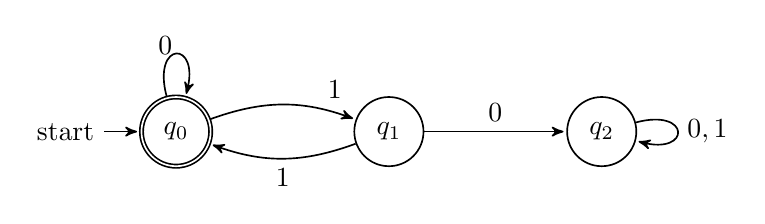
\begin{tikzpicture}[->,>=stealth',shorten >=1pt, auto, node distance=2cm, semithick]
\tikzstyle{every state}=[text=black, fill=none]

\node[initial,state, accepting] (q0)          {$q_0$};
\node[state]         (q1) [right of=q0, xshift=20pt] {$q_1$};
\node[state]         (q2) [right of=q1, xshift=20pt] {$q_2$};

\path (q0) edge  [loop above, near start] node {$0$} (q0)
        edge [bend left=20, near end] node {$1$} (q1)
    (q1) edge [bend left=0] node {$0$} (q2)
        edge [bend left=20] node {$1$} (q0)
    (q2) edge [loop right] node {$0,1$} (q2)
;
\end{tikzpicture}
\end{center}
where $Q = \{q_0, q_1, q_2\}$, $\Sigma = \{0,1\}$, and $F = \{q_0\}$, and $\delta: Q \times \Sigma \to Q$
is specified by the look-up table
\begin{center}
\begin{tabular}{c|cc}
        & $0$ & $1$ \\
    \hline
  $q_0$ & $q_0$ & $q_1$ \\
  $q_1$ & $q_2$ & $q_0$ \\
  $q_2$ & $q_2$ & $q_2$
\end{tabular}
\end{center}
    \begin{enumerate}
    \item\gradeComplete A friend tries to summarize the transition function with the formula
    \[
        \delta(q_i,x) = \begin{cases}
            q_0 &\text{ when $i=0$ and $x=0$} \\
            q_2 &\text{ when $x < i$}\\
            q_j &\text{ when $j = (i+1) \mod 2$ and $x=1$}
        \end{cases}
    \]
    for $x \in \{0,1\}$ and $i \in \{0,1,2\}$.
    Are they right? Either help them justify their claim or give a counterexample to disprove it and then 
    fix their formula.

    \item\gradeCorrect Give a regular expression $R$ so that $L(R)$ is the language 
    recognized by this finite automaton. Justify your answer by referring to the 
    definition of the semantics of regular expressions and computations of finite automata. 
    Include an explanation for why each string in $L(R)$ is accepted by the finite automaton {\it and}
    for why each string not in $L(R)$ is rejected by the finite automaton.

    \item\gradeCorrect Keeping the same set of states $Q = \{q_0, q_1, q_2\}$, alphabet $\Sigma = \{0,1\}$, 
    same start state $q_0$, and same transition 
    function $\delta$, choose a new set of accepting states $F_{new}$ so that the new 
    finite automaton that results accepts at least one string that the original one rejected {\bf and} rejects
    at least one string that the original one accepted, or explain why there is no such choice of $F_{new}$.
    A complete solution will include either (1) a precise and
    clear description of your choice of $F_{new}$
    and a precise and clear the two example strings using relevant definitions 
    to justify them, or (2) a sufficiently general and correct argument
    why there is no such example, referring back to the relevant definitions.

    \end{enumerate}
    
    \end{enumerate}
\newpage

\title{HW2CSE105F24: Homework assignment 2}
\date{Due: October 15th at 5pm, via Gradescope}



\maketitle
\thispagestyle{fancy}

{\bf In this assignment,}

You will practice designing multiple representations of regular languages and working with 
general constructions of automata to demonstrate the richness of the class of regular languages.


{\bf Resources}: To review the topics 
for this assignment, see the class material from Week 2.
We will post frequently asked questions and our answers to them in a 
pinned Piazza post. 

{\bf Reading and extra practice problems}:  
Sipser Section 1.1, 1.2, 1.3. 
Chapter 1 exercises 1.4, 1.5, 1.6, 1.7, 1.8, 1.9, 1.10, 1.11, 1.12, 1.14, 1.15, 
1.16, 1.17, 1.19, 1.20, 1.21, 1.22. Chapter 1 problem 1.51.

\instructions

You will submit this assignment via Gradescope
(\href{https://www.gradescope.com}{https://www.gradescope.com}) 
in the assignment called ``hw2CSE105F24''.

{\bf Assigned questions}
\begin{enumerate}[wide, labelwidth=!, labelindent=0pt]
%%%%%%%%%%% PROBLEM 1 %%%%%%%%%%%
\item \textbf{Automata design} (12 points):
As background to this question, recall that integers can be represented using base $b$ expansions, for 
any convenient choice of base $b$. The precise definition is:
for $b$ an integer greater than $1$ and $n$ a positive integer, 
the {\bf base $b$ expansion of $n$}  is defined to be
\[
(a_{k-1} \cdots a_1 a_0)_b
\]
where $k$ is a positive integer, $a_0, a_1, \ldots, a_{k-1}$ 
are nonnegative integers less than $b$, $a_{k-1} \neq  0$, and
\[
n =  \sum_{i=0}^{k-1} a_{i} b^{i}
\]

Notice: {\it The base $b$ expansion of a positive integer $n$ is a string over the alphabet 
$\{x \in \mathbb{Z} \st 0 \leq x < b\}$
whose leftmost character is nonzero.}

An important property of base $b$ expansions of integers is that, for each integer $b$ greater than $1$,
each positive integer $n = (a_{k-1} \cdots a_1 a_0)_b$, and each nonnegative integer $a$ less than $b$, 
\[
    bn + a = (a_{k-1} \cdots a_1 a_0a)_b
\]
In other words, shifting the base $b$ expansion to the left results in multiplying the integer value by the base.
In this question we'll explore building deterministic finite automata that recognize 
languages that correspond to useful sets of integers.

    \begin{enumerate}
    \item\gradeCompleteFirst Design a DFA that recognizes the set of binary (base $2$) expansions of 
    positive integers that are powers of $2$. A complete solution will include the state diagram of your DFA and 
    a brief justification 
    of your construction by explaining the role each state plays in the machine, as well as a brief 
    justification about how the strings accepted and rejected by the machine connect to the specified language.

    {\it Hints}: (1) A power of $2$ is an integer $x$ that can be written as $2^y$ for some nonnegative integer $y$, 
    (2) the DFA should accept the strings $100$, $10$ and $100000$ and should reject the 
    strings $010$, $1101$, and $\varepsilon$ (can you see why?).

    \item\gradeComplete Consider arbitrary positive integer $m$. Design a DFA that recognizes the 
    set of binary (base $2$) expansions of positive integers that are multiples of $m$. A complete solution will
    include the formal definition of your DFA (paramterized by $m$) and a brief justification of your 
    construction by explaining the role each state plays in the machine, as well as a brief 
    justification about how the strings accepted and rejected by the machine connect to the specified language.

    {\it Hints}: (1) Consider having a state for each possible remainder upon division by $m$.
     (2) To determine transitions, notice that reading a new character will shift what we already read over by
     one slot.

    \item\gradeCorrectFirst Choose a positive integer $m_{0}$ between $5$ and $8$ (inclusive) and draw the state diagram
    of a DFA recognizing the following language over $\{0,1,2,3\}$ 
    $$\{ w \in \{0,1,2,3\}^* \mid w \text{ is a base $4$ expansion of a positive 
    integer that is a multiple of $m_0$}\}$$
    A complete solution will include the state diagram of your DFA and 
    a brief justification 
    of your construction by explaining the role each state plays in the machine, as well as a brief 
    justification about how the strings accepted and rejected by the machine connect to the specified language.
    \end{enumerate}

    {\it Bonus extension to think about (ungraded):} Which other languages related to sets of integers 
    can be proved to be regular using a similar strategy? 

%%%%%%%%%%% PROBLEM 2 %%%%%%%%%%%
\item \textbf{Nondeterminism} (15 points): For this question, the alphabet is $\{a,b\}$.
\begin{enumerate}
\item\gradeComplete Design a DFA that recognizes the language
    \[ 
    \{w \in \{a,b\}^* \mid w \text{ contains at most one $a$ {\bf and} at least two $b$s}\}
    \]
    You can design this DFA directly or use the constructions from class (and the footnote to Theorem 
    1.25 in the book) to build this DFA from DFA for the simpler languages that are intersected
    to give this language.
    
    A complete solution will include the state diagram of your DFA and 
    a brief justification 
    of your construction either by explaining the role each state plays in the machine, as well as a brief 
    justification about how the strings accepted and rejected by the machine connect to the specified language, 
    or by justifying the design of the DFA for the simpler languages and then describing how the Theorem was used.


    \item\gradeCorrect Design a NFA with at most $6$ states that recognizes the language
\[ 
\{w \in \{a,b\}^* \mid w \text{ contains at most one $a$ {\bf and} at least two $b$s}\}
\]
A complete solution will include the state diagram of your NFA and 
    a brief justification 
    of your construction by explaining the role each state plays in the machine, as well as a brief 
    justification about how the strings accepted and rejected by the machine connect to the specified language.
    Give one example string in the language and explain the computation of the NFA
    that witnesses that the machine accepts this string.
    Also, give one example string not in the language and explain why the NFA rejects this string.

\item\gradeCorrect Design a NFA with at most $6$ states that recognizes the language
\[ 
\{w \in \{a,b\}^* \mid w \text{ contains at most one $a$ {\bf or} at least two $b$s}\}
\]
A complete solution will include the state diagram of your NFA and 
    a brief justification 
    of your construction by explaining the role each state plays in the machine, as well as a brief 
    justification about how the strings accepted and rejected by the machine connect to the specified language.
    Give one example string in the language and explain the computation of the NFA
    that witnesses that the machine accepts this string.
    Also, give one example string not in the language and explain why the NFA rejects this string.
\end{enumerate}
{\it Bonus extension to think about (ungraded):} Did you need all $6$ states? Could you design DFA with $6$ states that recognize
each of these langauges?

%%%%%%%%%%% PROBLEM 3 %%%%%%%%%%%
\item\textbf{General constructions} (15 points):
In this question, you'll practice working with formal general constructions
for NFAs and translating between state diagrams and formal definitions.

\begin{enumerate}
\item\gradeCorrect Consider the following general construction: Let $N_1 = (Q, \Sigma, \delta_1, q_1, F_1)$ be a NFA
and assume that $q_0 \notin Q$.
Define the new NFA $N_2 = (Q \cup \{q_0\}, \Sigma, \delta_2, q_0, \{q_1\})$ where 
$$\delta_2: (Q \cup \{q_0\}) \times \Sigma_\varepsilon \to \mathcal{P} (Q \cup \{q_0\})$$ is defined by
\[
    \delta_2 (q,a) = \begin{cases}
        \{ q' \in Q \mid q \in \delta_1(q',a)\} &\text{if $q \in Q$, $a \in \Sigma_{\varepsilon}$} \\
        F_1 &\text{if $q =q_0$, $a = \varepsilon$}\\
        \emptyset &\text{if $q = q_0$, $a \in \Sigma$}
    \end{cases}
\]
Illustrate this construction by defining a specific example NFA $N_1$ and applying the 
construction above to create the new NFA $N_2$. Your example NFA should
\begin{itemize}
    \item Have exactly four states (all reachable from the start state),
    \item Accept at least one string and reject at least one string, and
    \item Not have any states labelled $q_0$.
\end{itemize}
Apply the construction above to create the new NFA. A complete submission 
will include the state diagram of your example NFA $N_1$ and the state diagram of the NFA $N_2$ resulting 
from this construction and a precise and clear description of $L(N_1)$ and $L(N_2)$, justified
by explaining the role each state plays in the machine, as well as a brief 
justification about how the strings accepted and rejected by the machine connect to the language.

\item 
In Week 2's review quiz, we saw the definition that a set $X$ is said to be 
{\bf closed under an operation} if, for any elements in
$X$, applying to them gives an element in $X$. For example, the set of
integers is closed under multiplication because if we take any two
integers, their product is also an integer .

Recall the definitions we have: 
For each language $L$ over the alphabet $\Sigma_1 = \{0,1\}$, we have the 
associated set of strings
  $$EXTEND(L) = \{ w \in \Sigma_1^* ~|~ w = uv \text{ for some strings } u \in L \text{ and } v \in \Sigma_1^* \}$$
We will prove that the collection of languages over $\{0,1\}$ that are each 
recognizable by some NFA is closed under the $EXTEND$ operation.

\begin{enumerate}
 
   \item \gradeComplete As a helpful tool in our construction\footnote{A result that is proved in 
   order to work towards a larger theorem is called a Lemma.}, prove that every NFA can be 
   converted to an equivalent one that has a single accept state. Note: this is exercise 1.11 in 
   the textbook.

   \item \gradeCorrect Prove that the collection of languages over $\{0,1\}$ that are each 
   recognizable by some NFA is closed under the $EXTEND$ operation. You can assume 
   that you are given a NFA with a single accept state $N = (Q, \{0,1\}, \delta, q_0, \{q_{acc}\})$
   and you need to define a new NFA, $N_{new} = (Q_{new}, \{0,1\}, \delta_{new}, q_{new}, F_{new})$,
    so that $L(N_{new}) = EXTEND(L(N))$. 

    A complete solution will include precise definitions for $Q_{new}, \delta_{new}, q_{new},$ and 
    $F_{new}$, as well as a 
    a brief justification 
    of your construction by explaining why these definitions work, referring 
    specifically to the definition of $EXTEND$ and to acceptance of NFA.

\end{enumerate}

\end{enumerate}
%%%%%%%%%%% PROBLEM 4 %%%%%%%%%%%
\item\textbf{Multiple representations} (8 points):
For any language $L \subseteq \Sigma^*$, recall that we define its \emph{complement} as 
$$\overline{L} := \Sigma^* - L = \{w \in \Sigma^* \mid w \notin L\}$$ That is, the complement of $L$ 
contains all and only those strings which are not in $L$. Our notation for regular expressions does not 
include the complement symbol. However, 
it turns out that the complement of a language described by a regular expression is guaranteed to also be describable by a 
(different) regular expression.\footnote{We'll see that this is connected to the 
result we proved in class that the complement of each language recognizable by a DFA is 
recognizable by a(nother) DFA.}

For example, over the alphabet $\Sigma = \{a,b\}$, the complement of the language described 
by the regular expression $\Sigma^* b$ is described by the regular expression $\varepsilon \cup \Sigma^*a$
because any string that does not end in $b$
must either be the empty string or end in $a$.

For each of the regular expressions $R$ over the alphabet $\Sigma = \{a,b\}$ below, write the regular 
expression for~$\overline{L(R)}$. Your regular expressions may use the symbols
$\varnothing$, $\varepsilon$, $a$, $b$, and the 
following operations to combine them: union, concatenation, 
and Kleene star.

Briefly justify why your solution for each part works by giving plain English descriptions of the language 
described by the regular expression and of its complement and connecting them to the regular 
expression via relevant definitions. An English description that is more 
detailed than simply negating the description in the original language will likely be helpful in the justification.

Alternatively, you can justify your solution by first designing a DFA that recognizes $L(R)$, 
using the construction from class and the book to modify this DFA to get a new DFA that recognizes~$\overline{L(R)}$, 
and then applying the constructions from class and the book to convert this new DFA to a regular expression.

For each part of the question, clearly state which approach you're taking and include enough intermediate
steps to illustrate your work.


\begin{enumerate}
    \item\gradeCorrect $(a \cup b)^*a(a \cup b)^*$
    \item\gradeCorrect $(a \cup b) (a \cup b) (a \cup b)$
\end{enumerate}

\end{enumerate}
\newpage

\title{HW3CSE105F24: Homework assignment 3}
\date{Due: October 22nd at 5pm, via Gradescope}



\maketitle
\thispagestyle{fancy}

{\bf In this assignment,}

You will demonstrate the richness of the class of regular languages, as well as its boundaries.


{\bf Resources}: To review the topics 
for this assignment, see the class material from Week 3.
We will post frequently asked questions and our answers to them in a 
pinned Piazza post. 

{\bf Reading and extra practice problems}:  
Sipser Chapter 1.
Chapter 1 exercises 1.4, 1.5, 1.6, 1.7, 1.8, 1.9, 1.10, 1.11, 1.12, 1.14, 1.15, 
1.16, 1.17, 1.19, 1.20, 1.21, 1.22. Chapter 1 problem 1.51.

\instructions

You will submit this assignment via Gradescope
(\href{https://www.gradescope.com}{https://www.gradescope.com}) 
in the assignment called ``hw3CSE105F24''.

{\bf Assigned questions}
\begin{enumerate}[wide, labelwidth=!, labelindent=0pt]

%%%%%%%%%%% PROBLEM 1 %%%%%%%%%%%
\item \textbf{Using general constructions} (16 points): Consider the NFA $N$ over $\{0,1,2\}$ with state diagram


   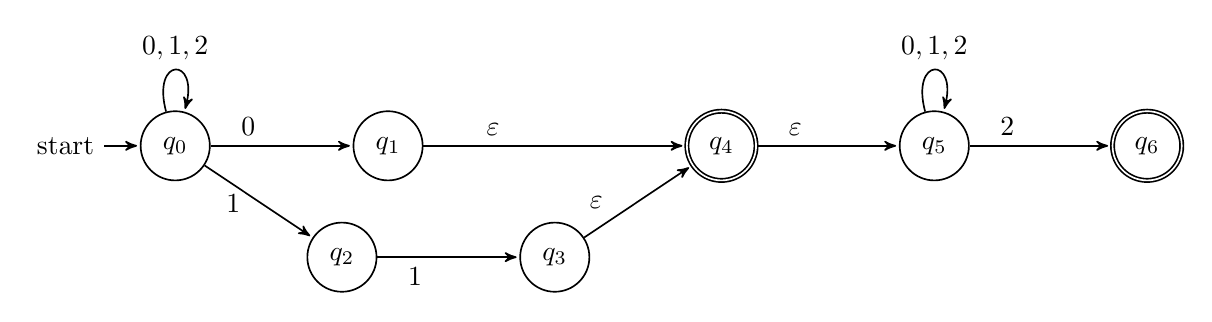
\begin{tikzpicture}[->,>=stealth',shorten >=1pt, auto, node distance=2cm, semithick]
   \tikzstyle{every state}=[text=black, fill=none]
   
   \node[initial,state] (q0)          {$q_0$};
   \node[state]         (q1) [right of=q0, xshift=20pt] {$q_1$};
   \node[state]         (q2) [below right of=q0, xshift=20pt] {$q_2$};
   \node[state]         (q3) [right of=q2, xshift=20pt] {$q_3$};
   \node[state, accepting]         (q4) [above right of=q3, xshift=20pt] {$q_4$};
   \node[state]         (q5) [right of=q4, xshift=20pt] {$q_5$};
   \node[state, accepting]         (q6) [right of=q5, xshift=20pt] {$q_6$};
   
   \path (q0) edge  [loop above] node {$0,1,2$} (q0)
           edge [bend right=0, near start] node[above] {$0$} (q1)
           edge [bend left=0, near start] node[below] {$1$} (q2)
       (q1) edge [bend left=0, near start] node {$\varepsilon$} (q4)
       (q2) edge [bend left=0, near start] node[below] {$1$} (q3)
       (q3) edge [bend left=0, near start] node {$\varepsilon$} (q4)
       (q4) edge [bend left=0, near start] node {$\varepsilon$} (q5)
       (q5) edge [loop above] node {$0,1,2$} (q5)
       (q5) edge [bend left=0, near start] node {$2$} (q6)
   ;
   \end{tikzpicture}

    \begin{enumerate}
      \item\gradeCompleteFirst Give two examples of strings of length greater than $2$ 
      that are accepted by $N$ and two examples of strings of length greater than $2$ 
      that are rejected by $N$. For each example string, list at least one of the 
      computations of $N$ on this string and 
      label whether this computation witnesses that the string is accepted by $N$.

      \item\gradeCorrectFirst Use the ``macro-state'' construction from Theorem 1.39 and class to create the DFA
      $M$ recognizing the same language as $N$. You only need to include states that are reachable from the start
      state. For full credit, submit (1) a state diagram that is deterministic (there should be arrows labelled $0$, $1$, and 
      $2$ coming out of each state) and where each state is labelled by a subset of the states in $N$; 
      and (2) for one of your example strings that is accepted by $N$, give the computation of $M$ on this string as a 
      seqeuence of states visited; and (3) for one of your example strings that is rejected by $N$, 
      give the computation of $M$ on this string as a seqeuence of states visited.

      \item\gradeComplete Give a mathematical description either using set builder notation or a regular expression
      for $L(N)$ and for $L(M)$.
    \end{enumerate}

%%%%%%%%%%% PROBLEM 2 %%%%%%%%%%%
\item \textbf{Multiple representations} (12 points):

\begin{enumerate}
   \item Consider the language $A_1 = \{ uw \mid \text{$u$ and
   $w$ are strings over $\{0,1\}$ and have the same length} \}$
   and the following argument.

   \begin{quote}
      ``Proof" that $A_1$ is not regular using the Pumping Lemma: Let $p$ be 
      an arbitrary positive integer. We will show that $p$ is not a pumping length for $A_1$. 
      
      Choose $s$ to be the string $1^p 0^p$, which is in $A_1$ because
      we can choose $u = 1^p$ and $w = 0^p$ which each have length $p$.
      Since $s$ is in $A_1$ and has length greater than or equal to $p$, if $p$ were to be a
      pumping length for $A_1$, $s$ ought to be pump'able. 
      That is, there should be a way of dividing $s$ into parts $x,y,z$ where $s=xyz$,
      $|y| >0$, $|xy| \leq p$, and for each $i \geq 0$, $xy^iz \in A_1$.
      Suppose $x,y,z$ are such that $s = xyz$, $|y| > 0$ and $|xy| \leq p$.
      Since the first $p$ letters of $s$ are all $1$ and $|xy| \leq p$, we know
      that $x$ and $y$ are made up of all $1$s.  If we let $i=2$, we get 
      a string $xy^iz$ that is not in $A_1$ because repeating $y$ twice adds $1$s to 
      $u$ but not to $w$, and strings in $A_1$ are required to have $u$ and $w$ be the same
      length. Thus, $s$ is not pumpable (even though it should have been if $p$ were to be a pumping length)
      and so $p$ is not a pumping length for $A_1$.  Since $p$ was arbitrary, we have
      demonstrated that $A_1$ has no pumping length.  By the Pumping Lemma, this implies that 
      $A_1$ is nonregular.
      \end{quote}
      \begin{enumerate}
         \item \gradeComplete Find the (first and/or most significant) logical error in the ``proof" above 
         and describe why it's wrong.
   
         \item \gradeComplete Prove that the set $A_1$ is actually regular (by finding a regular expression that describes it or 
         a DFA/NFA that recognizes it, and justifying why) {\bf or} fix the proof so that it is logically sound.     
      \end{enumerate}

   \item Consider the language $A_2 = \{ u1w \mid \text{$u$ and
   $w$ are strings over $\{0,1\}$ and have the same length} \}$
   and the following argument.


   \begin{quote}
      ``Proof" that $A_2$ is not regular using the Pumping Lemma: Let $p$ be 
      an arbitrary positive integer. We will show that $p$ is not a pumping length for $A_2$. 
      
      Choose $s$ to be the string $1^{p+1} 0^{p}$, which is in $A_2$ because
      we can choose $u = 1^p$ and $w = 0^p$ which each have length $p$.
      Since $s$ is in $A_2$ and has length greater than or equal to $p$, if $p$ were to be a
      pumping length for $A_2$, $s$ ought to be pump'able. 
      That is, there should be a way of dividing $s$ into parts $x,y,z$ where $s=xyz$,
      $|y| >0$, $|xy| \leq p$, and for each $i \geq 0$, $xy^iz \in A_2$.
      When $x = \varepsilon$ and $y = 1^{p+1}$ and $z = 0^{p}$,
      we have satisfied that $s = xyz$, $|y| > 0$ (because $p$ is positive) and $|xy| \leq p$.
      If we let $i=0$, we get 
      the string $xy^iz = 0^{p}$ that is not in $A_2$ because its middle symbol is a $0$, not a $1$. 
      Thus, $s$ is not pumpable (even though it should have been if $p$ were to be a pumping length)
      and so $p$ is not a pumping length for $A_2$.  Since $p$ was arbitrary, we have
      demonstrated that $A_2$ has no pumping length.  By the Pumping Lemma, this implies that 
      $A_2$ is nonregular.
      \end{quote}

      \begin{enumerate}

      \item \gradeComplete Find the (first and/or most significant) logical error in the ``proof" above 
      and describe why it's wrong.

      \item \gradeComplete Prove that the set $A_2$ is actually regular (by finding a regular expression that describes it or 
      a DFA/NFA that recognizes it, and justifying why) {\bf or} fix the proof so that it is logically sound.
      
      \end{enumerate}
   
\end{enumerate}


%%%%%%%%%%% PROBLEM 3 %%%%%%%%%%%
\item \textbf{Pumping} (10 points):

\begin{enumerate}
\item\gradeCorrect Give an example of a language
over the alphabet $\{a,b\}$ that has cardinality $5$ and for which $4$ is a pumping length
and $3$ is not a pumping length. Is this language regular? A complete solution will give 
(1) a clear and precise
description of the language, (2) a justification for why $4$ is a pumping length, (3) a 
justification for why $3$ is not a pumping length, (4) a correct and justified answer to 
whether the language is regular.


\item\gradeComplete In class and in the reading so far, we've seen the following examples of nonregular sets:
\begin{multicols}{3}
\begin{center}
$\{ 0^n 1^n ~|~ n \geq 0 \}$
$$\{ 0^n 1^n ~|~ n \geq 2 \}$$
$$\{ 0^n 1^m ~|~  0 \leq n \leq m \}$$
$$\{ 0^n 1^m ~|~ 0 \leq m \leq n \}$$
$$\{ 0^i 1^{2i} ~|~ 0 \leq i \}$$
$$\{ 0^i 1^{i+1} ~|~ 0 \leq i \}$$
$$\{ 0^n 1^m 0^n ~|~n,m \geq 0\}$$
$$\{ w \in \{0,1\}^* ~|~w = w^R\}$$
$$\{ w w^R ~|~ w \in \{0,1\}^*\}$$
\end{center}
\end{multicols}
Modify one of these sets in some way and use the Pumping Lemma to prove that the resulting set is still nonregular.

\end{enumerate}

%%%%%%%%%%% PROBLEM 4 %%%%%%%%%%%
\item\textbf{Regular and nonregular languages} (12 points):
In Week 2's review quiz, we saw the definition that a set $X$ is said to be 
{\bf closed under an operation} if, for any elements in
$X$, applying to them gives an element in $X$. For example, the set of
integers is closed under multiplication because if we take any two
integers, their product is also an integer .

Prove or disprove each closure claim statement below about the class of regular languages
and the class of nonregular languages.
Your arguments may refer to theorems proved in the textbook and class, and if they do, should 
include specific page numbers and references (i.e.\ write out the claim that was proved in the book 
and/or class).

Recall the definitions we have: 

For language $L$ over the alphabet $\Sigma_1 = \{0,1\}$, we have the 
associated sets of strings
\[
   SUBSTRING(L) = \{ w \in \Sigma_1^* ~|~ \text{there exist } a,b \in \Sigma_1^* \text{ such that } awb \in L\}
\]
and 
\[
  EXTEND(L) = \{ w \in \Sigma_1^* ~|~ w = uv \text{ for some strings } u \in L \text{ and } v \in \Sigma_1^* \}
\]
\begin{enumerate} 
   \item \gradeComplete The set of regular languages over $\{0,1\}$ is closed under the $SUBSTRING$ operation.

   \item \gradeComplete The set of nonregular languages over $\{0,1\}$ is closed under the $SUBSTRING$ operation.

   \item \gradeCorrect The set of regular languages over $\{0,1\}$ is closed under the $EXTEND$ operation.

   \item \gradeCorrect The set of nonregular languages over $\{0,1\}$ is closed under the $EXTEND$ operation.
\end{enumerate}

\end{enumerate}
\newpage

\title{HW4CSE105F24: Homework assignment 4}
\date{Due: November 12, 2024 at 5pm, via Gradescope}



\maketitle
\thispagestyle{fancy}

{\bf In this assignment,}

You will work with context-free languages and their representations.
You will  also practice analyzing, designing, and working with Turing machines.
You will use general constructions and specific machines to explore the classes 
of recognizable and decidable languages.


{\bf Resources}: To review the topics 
for this assignment, see the class material from Weeks 4, 5, and 6.
We will post frequently asked questions and our answers to them in a 
pinned Piazza post. 

{\bf Reading and extra practice problems}:  
Sipser Chapters 2 and 3.
Chapter 2 exercises 2.1, 2.2, 2.3, 2.4, 2.5, 2.6, 2.7, 2.9, 2.10, 2.11, 2.12, 2.13, 2.16, 2.17.
Chapter 3 exercises 3.1, 3.2, 3.5, 3.8.

\instructions

You will submit this assignment via Gradescope
(\href{https://www.gradescope.com}{https://www.gradescope.com}) 
in the assignment called ``hw4CSE105F24''.

{\bf Assigned questions}
\begin{enumerate}[wide, labelwidth=!, labelindent=0pt]

%%%%%%%%%%% PROBLEM 1 %%%%%%%%%%%
\item \textbf{Push-down automata (PDA) and context-free grammars (CFG)} (8 points): 
On page 14 of the week 3 notes, we have the following list of languages over the alphabet $\{a,b\}$

\begin{center}
\begin{tabular}{ccc}
    $\{a^nb^n \mid 0  \leq n  \leq 5 \}$
    &$\{b^n a^n \mid  n  \geq 2\}$
    &$\{a^m b^n \mid  0 \leq m\leq n\}$
\end{tabular}
\begin{tabular}{cc}
    $\{a^m b^n \mid  m \geq n+3,  n \geq 0\}$
    &$\{b^m a^n \mid  m \geq 1, n \geq  3\}$\\
    $\{ w  \in \{a,b\}^* \mid w = w^\mathcal{R} \}$
    &$\{ ww^\mathcal{R} \mid w\in \{a,b\}^* \}$ \\
\end{tabular}
\end{center}
\begin{enumerate}
    \item\gradeCompleteFirst Pick one of the regular languages and design a regular expression that describes it. 
    Briefly justify your regular expression by connecting
    the subexpressions of it to the intended language and referencing relevant definitions.
    \item\gradeComplete Pick another one of the regular languages and design a deterministic finite automaton (DFA) that recognizes it. Draw the 
    state diagram of your DFA. Briefly justify your design by explaining the role each state plays in the machine, 
    as well as a brief 
    justification about how the strings accepted and rejected by the machine connect to the specified language.
    \item\gradeComplete Pick one of the nonregular languages and design a PDA that recognizes it. Draw the state diagram of 
    your PDA. Briefly justify your design by explaining the role each state plays in the machine, 
    as well as a brief 
    justification about how the strings accepted and rejected by the machine connect to the specified language.
    \item\gradeComplete Pick one of the nonregular languages and write a CFG that generates it. Briefly justify
    your design by demonstrating how derivations in the grammar relate
    to the intended language.
\end{enumerate}

%%%%%%%%%%% PROBLEM 2 %%%%%%%%%%%
\item \textbf{General constructions for context-free languages} (21 points):

In class in weeks 4 and 5, we described several general constructions 
with PDAs and CFGs, leaving their details to
homework. In this question, we'll fill in these details. The first constructions
help us prove that the class of regular languages is a subset of the
class of context-free languages. The other construction allows us 
to make simplifying assumptions about PDAs recognizing languages.

\begin{enumerate}

\item\gradeCorrectFirst When we first introduced PDAs we observed 
that any NFA can be transformed to a PDA by not using the stack 
of the PDA at all. Suppose a friend gives you the following construction
to formalize this transformation:

\begin{quote}
Given a NFA $N = (Q, \Sigma, \delta_N, q_0, F)$ we define a PDA $M$
with $L(M) = L(N)$ by letting $M = ( Q, \Sigma, \Sigma, \delta, q_0, F)$ where 
$\delta(~(q,a,b)~) = \delta_N(~(q,a)~)$ for each $q \in Q$, 
$a \in \Sigma_{\varepsilon}$ and $b \in \Sigma_{\varepsilon}$.
\end{quote}

For each of the six defining parameters for the PDA, explain whether 
it's defined correctly or not. If it is not defined correctly, 
explain why not and give a new definition for this parameter that 
corrects the mistake.

\item\gradeCorrect In the book on page 107, the top paragraph describes a procedure for converting DFAs to CFGs:
\begin{quote}
   You can convert any DFA into an equivalent CFG as follows. 
   Make a variable $R_i$ for each state $q_i$ of the DFA. Add the rule $R_i \to aR_j$ to the
   CFG if $\delta(q_i,a) =q_j$ is a transition in the DFA. Add the rule
   $R_i\to \varepsilon$ if $q_i$ is an accept state of the DFA. Make $R_0$ the start variable ofthe grammar, 
   where $q_0$ is the start state of the machine. Verify on your own that the resulting CFG 
   generates the same language that the DFA recognizes.
\end{quote}

Use this construction to get a context-free grammar generating the language 
\[
    \{ w \in \{0,1\}^* \mid w \text{ does not end in  $101$}\}
\]
by (1) designing a DFA that recognizes this language and then (2) applying the construction from the book to convert the 
DFA to an equivalent CFG. A complete and correct submission will include the state diagram of the DFA, a brief justification of why 
it recognizes the language, and then the complete and precise definition of the CFG that results from applying the construction 
from the book to this DFA. {\it Ungraded bonus: take a sample string in the language and see how the computation of 
the DFA on this string translates to a derivation in your grammar.}

\item Let $M_1 = (Q_1, \Sigma, \Gamma_1, \delta_1, q_1, F_1)$ 
be a PDA and let $q_{new}, r_{new}, s_{new}$ be three fresh state labels 
(i.e. $Q_1 \cap \{q_{new}, r_{new}, s_{new}\} = \emptyset$) 
and let $\#$ be a fresh stack symbol (i.e. $\# \notin \Gamma_1$).
We define the PDA $M_2$ as
\[
   (Q_2, \Sigma, \Gamma_2, \delta_2, q_{new}, \{s_{new}\})
\]
with $Q_2 = Q_1 \cup \{q_{new}, r_{new}, s_{new}\}$ 
and $\Gamma_2 = \Gamma_1 \cup \{\#\}$
and 
$\delta_2 : Q_2 \times \Sigma_\varepsilon \times {\Gamma_2}_\varepsilon \to 
\mathcal{P}(Q_2 \times {\Gamma_2}_\varepsilon)$ given by 
\[
\delta_2 ( ~(q,a,b)~) = 
\begin{cases}
\{(q_1, \#)\} &\text{if } q = q_{new}, a = \varepsilon, b = \varepsilon\\
\delta_1( ~(q,a,b)~) &\text{if } q\in Q_1 \setminus F_1, a \in \Sigma_{\varepsilon}, b \in {\Gamma_1}_\varepsilon \\
\delta_1( ~(q,a,b)~) &\text{if } q\in F_1, a \in \Sigma, b \in {\Gamma_1}_\varepsilon \\
\delta_1( ~(q,a,b)~) &\text{if } q\in F_1, a =\varepsilon, b \in {\Gamma_1} \\
\delta_1( ~(q,a,b)~) \cup \{(r_{new}, \varepsilon)\} &\text{if } q\in F_1, a =\varepsilon, b =\varepsilon \\
\{(r_{new}, \varepsilon)\} &\text{if } q = r_{new}, a =\varepsilon, b \in \Gamma_{1} \\
\{(s_{new}, \varepsilon)\} &\text{if } q= r_{new}, a = \varepsilon, b = \#\\
\emptyset & \text{otherwise}
\end{cases}
\]
for each $q \in Q_2$, $a \in \Sigma_{\varepsilon}$, 
and $b \in {\Gamma_2}_\varepsilon$.

In this question, we'll apply this construction for a specific PDA and 
use this example to extrapolate the effect of this construction.
\begin{enumerate}

\item\gradeCorrect Consider the PDA $M_1$ with input alphabet $\{0,1\}$ 
and stack alphabet $\{0,1\}$ whose state diagram is

\begin{center}

   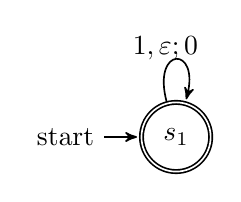
\begin{tikzpicture}[->,>=stealth',shorten >=1pt, auto, node distance=2cm, semithick]
      \tikzstyle{every state}=[text=black, fill=none]
    
    \node[initial,state, accepting] (s1)          {$s_1$};

    \path (s1) edge  [loop above, near start] node {$1,\varepsilon; 0$} (s1)
    ;
    \end{tikzpicture}
\end{center}

Draw the state diagram for the PDA $M_2$ that results from applying 
the construction to $M_1$.

\item\gradeComplete Compare $L(M_1)$ and $L(M_2)$. Are these sets 
equal? Does your answer depend on the specific choice of $M_1$? Why or why not?

\item\gradeComplete Consider the PDA $N$ with input alphabet $\{0,1\}$ and
stack alphabet $\{0,1\}$ whose state diagram is 

\begin{center}
   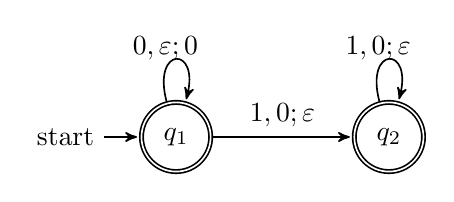
\begin{tikzpicture}[->,>=stealth',shorten >=1pt, auto, node distance=2cm, semithick]
      \tikzstyle{every state}=[text=black, fill=none]
    
    \node[initial,state, accepting] (q1)          {$q_1$};
    \node[state, accepting]         (q2) [right of=q1, xshift=20pt] {$q_2$};
    
    \path (q1) edge  [loop above, near start] node {$0,\varepsilon; 0$} (q1)
        (q1) edge [bend left=0] node {$1,0;\varepsilon$} (q2)
        (q2) edge [loop above, near start] node {$1,0;\varepsilon$} (q2)
    ;
    \end{tikzpicture}

\end{center}

   Remember that the definition of set-wise concatenation is:
    for languages $L_1, L_2$ over the alphabet $\Sigma$, we have the 
    associated set of strings
    \[
       L_1 \circ L_2 = \{ w \in \Sigma^* ~|~ w = uv \text{ for some strings } u \in L_1 \text{ and } v \in L_2 \}
    \]
    In class, we discussed how extrapolating the construction that we used to prove that the class of regular languages
    is closed under set-wise concategation by drawing 
    spontaneous transitions from the accepting states in the first 
    machine to the start state of the second machine doesn't work.
    Use the example of $M_1$ and $N_1$ to prove this by showing that
    \[
    L(M_1) \circ L(N)
    \]
    is {\bf not} the language recognized by the machine 
    results from taking the two machines
    $M_1$ and $N$, setting the start state of $M_1$ to be the start state of 
    the new machine, setting the set of accepting states of $N$ to be
    the set of accepting states of the new machine, and drawing spontaneous 
    arrows from the accepting states
    of $M_1$ to the start state of $N$.

    \item\gradeComplete Describe the language recognized by the machine 
    that results from taking the two machines
    $M_2$ and $N$, setting the start state of $M_2$ to be the start state of 
    the new machine, setting the set of accepting states of $N$ to be
    the set of accepting states of the new machine, and drawing spontaneous 
    arrows from the accepting states
    of $M_2$ to the start state of $N$. Use this description 
    to explain why we used the construction of $M_2$ from $M_1$
    and how this construction could be used in a proof of the 
    closure of the class of context-free languages under set-wise concatenation.
\end{enumerate}

\end{enumerate}
%%%%%%%%%%% PROBLEM 3 %%%%%%%%%%%
\item \textbf{Turing machines} (12 points):

Consider the Turing machine $T$ over the input alphabet $\Sigma = \{0,1\}$ with  the state
    diagram below (the tape alphabet is $\Gamma = \{ 0,1,X,\square\}$).  
    Convention: we do not include the node for the reject state $qrej$ and any missing transitions in the state diagram have value $(qrej,\square,R)$
    \begin{center}
      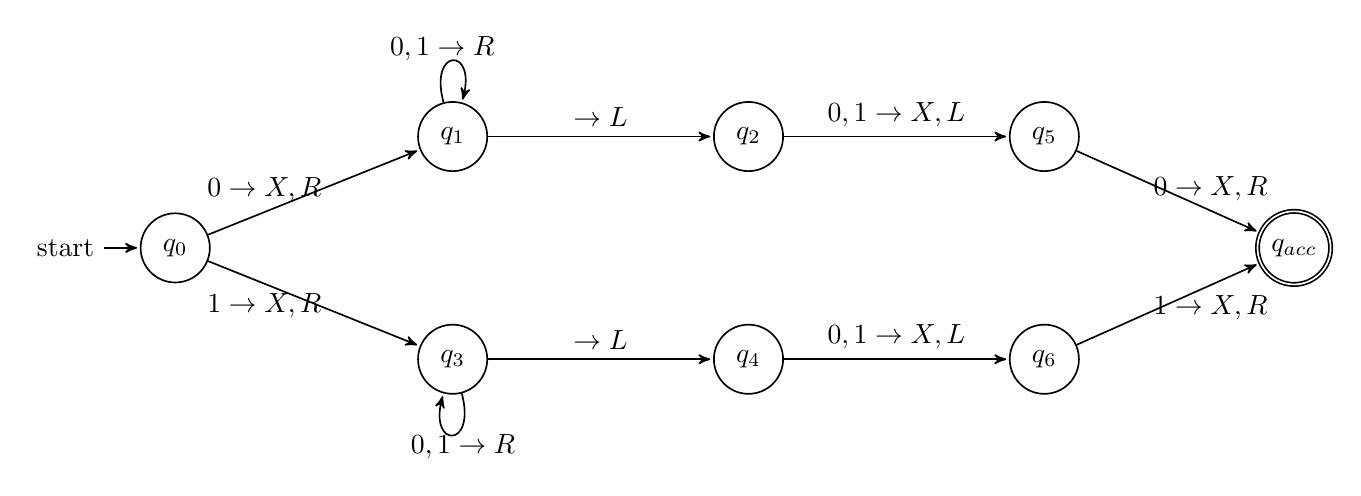
\begin{tikzpicture}[->,>=stealth',shorten >=1pt, auto, node distance=2cm, semithick]
         \tikzstyle{every state}=[text=black, fill=none]
        
        \node[initial,state] (q0)          {$q_0$};
        \node[state] (q1)  [above right of=q0, xshift=60pt] {$q_{1}$};
        \node[state] (q2)  [right of=q1, xshift=50pt] {$q_{2}$};
        \node[state] (q3)  [below right of=q0, xshift=60pt] {$q_{3}$};
        \node[state] (q4)  [right of=q3, xshift=50pt] {$q_{4}$};
        \node[state] (q5)  [right of=q2, xshift=50pt] {$q_5$};
        \node[state] (q6)  [right of=q4, xshift=50pt] {$q_6$};
        \node[state, accepting]         (qacc) [below right of=q5, xshift=50pt] {$q_{acc}$};
        
        \path (q1) edge  [loop above, near start] node {$0,1 \to R$} (q1)
            (q3) edge  [loop below, near start] node {$0,1 \to R$} (q3)
            (q0) edge [bend left=0, above, near start] node {$0\to X, R$} (q1)
            (q0) edge [bend left=0, below, near start] node {$1\to X, R$} (q3)
            (q1) edge [bend left=0] node {$\square \to L$} (q2)
            (q3) edge [bend left=0] node {$\square \to L$} (q4)
            (q2) edge [bend left=0] node {$0,1 \to X, L$} (q5)
            (q4) edge [bend left=0] node {$0,1 \to X, L$} (q6)
            (q5) edge [bend left=0, above, near end] node {$0\to X, R$} (qacc)
            (q6) edge [bend left=0, below, near end] node {$1\to X, R$} (qacc)
        ;
        \end{tikzpicture}
    \end{center}

    \begin{enumerate}

        \item\gradeCorrect Specify an example string $w_1$ of length $4$ over 
        $\Sigma$ that is {\bf accepted} by this Turing machine, or explain why there is no such 
        example. A complete solution will include either (1) a precise and clear 
        description of your example  string and a precise and clear description of the accepting computation
        of the Turing machine on this string or (2) a sufficiently
        general and correct argument why there is no such example, referring back to the relevant definitions.
        
        To describe a computation of a Turing machine, include the contents of the 
        tape, the state of the machine, and the location of the read/write head at each step in the computation.
        
        {\it Hint:} In class we've drawn pictures to represent the configuration of the machine at each step 
        in a computation.  You may do so or you may choose to describe these configurations in words.
        
        \item\gradeCorrect Specify an example string $w_2$ of length $3$ over $\Sigma$ 
        that is {\bf rejected} by this Turing machine
        or explain why there is no such 
        example. A complete solution will include either (1) a precise and clear 
        description of your example  string and a precise and clear description of the rejecting computation
        of the Turing machine on this string or (2) a sufficiently
        general and correct argument why there is no such example, referring back to the relevant definitions.

        \item\gradeCorrect Specify an example string $w_3$ of length $2$ over $\Sigma$ 
        on which  the computation of this Turing machine is {\bf never halts}
        or explain why there is no such 
        example. A complete solution will include either (1) a precise and clear 
        description of your example  string and a precise and clear description of the looping (non-halting) 
        computation
        of the Turing machine on this string or (2) a sufficiently
        general and correct argument why there is no such example, referring back to the relevant definitions.

        {\it Note}: when a Turing machine does not halt on a given input string, 
        we say that it {\bf loops} on that string.

\end{enumerate}



%%%%%%%%%%% PROBLEM 4 %%%%%%%%%%%
\item\textbf{Implementation-level descriptions of deciders and recognizers} (9 points):

For this question, consider the alphabet $\Sigma = \{a,b,c\}$.
\begin{enumerate}
\item[(a)]\gradeCorrect Give an example of an infinite language over $\Sigma$ (that is not $\Sigma^*$) and give
two different Turing machines that recognize it: one that is a decider and one that is not.
A complete solution will include a precise definition for your example language, 
along with {\bf both} a state diagram and an implementation-level description 
of each Turing machines, along with a brief explanation of why each of them recognizes
the language and why one is a decider and there other is not.

\item[(b)]\gradeComplete True or false: There is a Turing machine that is not a decider that recognizes 
the empty set. A complete solution will include a witness Turing machine (given by 
state diagram or implementation-level description or high-level description) and a justification 
for why it's not a decider and why it does not accept any strings, or a complete and correct
justification for why there is no such Turing machine.

\item[(c)]\gradeComplete True or false: There is a Turing machine that is not a decider that recognizes 
the set of all string $\Sigma^*$.  A complete solution will include a witness Turing machine 
(given by 
state diagram or implementation-level description or high-level description) and a justification 
for why it's not a decider and why it accept each string over $\{a,b,c\}$, or a complete and correct
justification for why there is no such Turing machine.
\end{enumerate}
\end{enumerate}
\newpage

\title{HW5CSE105F24: Homework assignment 5}
\date{Due: November 19, 2024 at 5pm, via Gradescope}



\maketitle
\thispagestyle{fancy}

{\bf In this assignment,}

You will  practice analyzing, designing, and working with Turing machines.
You will use general constructions and specific machines to explore the classes 
of recognizable and decidable languages. 
You will explore various ways to encode machines as strings so that 
computational problems can be recognized.

{\bf Resources}: To review the topics 
for this assignment, see the class material from Weeks 6 and 7.
We will post frequently asked questions and our answers to them in a 
pinned Piazza post. 

{\bf Reading and extra practice problems}:  
Sipser Sections 3.1, 3.3, 4.1
Chapter 3 exercises 3.1, 3.2, 3.5, 3.8.
Chapter 4 exercises 4.1, 4.2, 4.3, 4.4, 4.5.

\instructions

You will submit this assignment via Gradescope
(\href{https://www.gradescope.com}{https://www.gradescope.com}) 
in the assignment called ``hw5CSE105F24''.

{\bf Assigned questions}
\begin{enumerate}[wide, labelwidth=!, labelindent=0pt]

%%%%%%%%%%% PROBLEM 1 %%%%%%%%%%%
\item\textbf{Classifying languages} (10 points):
Our first example of a more complicated Turing machine was of a Turing machine 
that recognized the language $\{w \# w \mid w \in\{0,1\}^*\}$, which we 
know is not context-free. Let's call that Turing machine $M_0$. The language
\[
    L = \{ww \mid w \in \{0,1\}^*\}
\]
is also not context-free. 

\begin{enumerate}
    \item\gradeCorrectFirst Choose an example string of length $4$ in $L$ that is in {\bf not} in $\{w \# w \mid w \in\{0,1\}^*\}$ and describe the computation of the Turing machine $M_0$ on your example string. 
    Include the contents of the  tape, the state of the machine, and the location of the read/write head at each step in the computation.
    \item\gradeCompleteFirst Explain why the Turing machine from the textbook 
    and class that recognized $\{w \# w \mid w \in\{0,1\}^*\}$ does 
    not recognize $\{ww \mid w \in \{0,1\}^*\}$. Use your example to explain why $M_0$ doesn't recognize $L$.
    \item\gradeComplete Explain how you would change $M_0$ to get a 
    new Turing machine that does recognize $L$. Describe this new Turing machine using both an implementation-level definition and a state diagram of the Turing machine. You may use all 
    our usual conventions for state diagrams of Turing machines 
    (we do not include the node for the reject state $qrej$ and any missing transitions 
    in the state diagram have value $(qrej,\square,R)$; 
    $b \to R$ label means $b \to b, R$ ).
\end{enumerate}

%%%%%%%%%%% PROBLEM 2 %%%%%%%%%%%
\item\textbf{Closure} (18 points):
Suppose $M$ is a Turing machine over the alphabet $\{0,1\}$. 
Let $s_1, s_2, \ldots$ be a list of all strings in 
$\{0,1\}^*$ in string (shortlex) order.
We define a new Turing machine 
by giving its high-level description as follows: 
\begin{align*}
   M_{new} &= ``\text{On input }w:\\
    &\text{1. For $n = 1, 2, \ldots$}\\
    &\text{2.~~~For $j = 1, 2, \ldots n$} \\
    &\text{3.~~~For $k = 1, 2, \ldots, n$} \\
    &\text{4.~~~~~~Run the computation of $M$ on $s_jws_k$}\\
    &\text{5.~~~~~~If it accepts, accept.}\\
    &\text{6.~~~~~~If it rejects, go to the next iteration of the loop"}\\
\end{align*}

Recall the definitions we have:   For each language $L$ over the alphabet $\Sigma_1 = \{0,1\}$, we have the 
associated sets of strings
  $$SUBSTRING(L) = \{ w \in \Sigma_1^* ~|~ \text{there exist } x,y \in \Sigma_1^* \text{ such that } xwy \in L\}$$
and 
  $$EXTEND(L) = \{ w \in \Sigma_1^* ~|~ w = uv \text{ for some strings } u \in L \text{ and } v \in \Sigma_1^* \}$$

\begin{enumerate}
\item[(a)]\gradeCorrect Prove that this Turing machine construction 
{\bf cannot} be used to prove that the
class of decidable languages over $\{0,1\}$ is closed under the 
$EXTEND$ operation.
A complete and correct answer will give a counterexample which is a set $A$ over $\Sigma_1$ that  is decidable, along with a definition of Turing machine $M_A$ 
that decides $A$ 
(with a justification why this Turing machine accepts all 
strings in $A$ and rejects all strings not in $A$), and then either a description of the language of $M_{new}$ that results when setting the Turing machine $M = M_A$ and an explanation why $L(M_{new}) \neq EXTEND(A)$ or 
a description why $M_{new}$ is not a decider and therefore can't witness that $EXTEND(A)$ is decidable.

\item[(b)] \gradeCorrect Prove that this Turing machine construction cannot be used to prove that the
class of recognizable languages over $\{0,1\}$ is closed under the $SUBSTRING$ set operation. A complete and correct answer will 
give a counterexample of a specific language $B$ and Turing machine $M_B$ 
recognizing it
(with a justification why this Turing machine accepts all and only strings in $B$), and then a description of the language of $M_{new}$ that results when 
setting the Turing machine $M = M_B$ and an explanation why $L(M_{new}) \neq SUBSTRING(B)$

\item[(c)] \gradeComplete Define a new construction by slightly modifiying this one that can be used to prove  that the
class of recognizable languages over $\{0,1\}$ is closed under $SUBSTRING$. Justify that 
your construction works. The proof of correctness for the closure claim can be structured like: 
``Let $L_1 $ be a recognizable language over $\{0,1\}$ and 
assume we are given a Turing machine $M_1$ so that $L(M_1) = L_1$. Consider the new Turing machine 
$M_{new}$ defined above. We will show that $L(M_{new}) = SUBSTRING(L_1) $... {\it complete the proof
by proving subset inclusion in two directions, by tracing the relevant Turing machine computations}''

\item[(d)] \gradeComplete Prove that the class of recognizable languages over 
$\{0,1\}$ is closed under $EXTEND$.
\end{enumerate}

%%%%%%%%%%% PROBLEM 3 %%%%%%%%%%%
\item \textbf{Computational problems} (12 points):
Recall the definitions of some example computational problems from class

\hspace{-30pt}
    \begin{tabular}{|lcl|}
    \hline
    \multicolumn{3}{|l|}{{\bf  Acceptance problem} } \\
    & & \\
    \ldots for DFA & $A_{DFA}$ & $\{ \langle B,w \rangle \mid  \text{$B$ is a  DFA that accepts input 
    string $w$}\}$ \\
    \ldots for NFA & $A_{NFA}$ & $\{ \langle B,w \rangle \mid  \text{$B$ is a  NFA that accepts input 
    string $w$}\}$ \\
    \ldots for regular expressions & $A_{REX}$ & $\{ \langle R,w \rangle \mid  \text{$R$ is a  regular
    expression that generates input string $w$}\}$ \\
    \ldots for CFG & $A_{CFG}$ & $\{ \langle G,w \rangle \mid  \text{$G$ is a context-free grammar 
    that generates input string $w$}\}$ \\
    \ldots for PDA & $A_{PDA}$ & $\{ \langle B,w \rangle \mid  \text{$B$ is a PDA that accepts input string $w$}\}$ \\
    & & \\
    \hline
    \multicolumn{3}{|l|}{{\bf Language emptiness  testing} } \\
    & & \\
    \ldots for DFA & $E_{DFA}$ & $\{ \langle A \rangle \mid  \text{$A$ is a  DFA and  $L(A) = \emptyset$\}}$ \\
    \ldots for NFA & $E_{NFA}$ & $\{ \langle A\rangle \mid  \text{$A$ is a NFA and  $L(A) = \emptyset$\}}$ \\
    \ldots for regular expressions & $E_{REX}$ & $\{ \langle R \rangle \mid  \text{$R$ is a  regular
    expression and  $L(R) = \emptyset$\}}$ \\
    \ldots for CFG & $E_{CFG}$ & $\{ \langle G \rangle \mid  \text{$G$ is a context-free grammar 
    and  $L(G) = \emptyset$\}}$ \\
    \ldots for PDA & $E_{PDA}$ & $\{ \langle A \rangle \mid  \text{$A$ is a PDA and  $L(A) = \emptyset$\}}$ \\
    & & \\
    \hline
    \multicolumn{3}{|l|}{{\bf Language equality testing} } \\
    & & \\
    \ldots for DFA & $EQ_{DFA}$ & $\{ \langle A, B \rangle \mid  \text{$A$ and $B$ are DFAs and  $L(A) =L(B)$\}}$\\
    \ldots for NFA & $EQ_{NFA}$ & $\{ \langle A, B \rangle \mid  \text{$A$ and $B$ are NFAs and  $L(A) =L(B)$\}}$\\
    \ldots for regular expressions & $EQ_{REX}$ & $\{ \langle R, R' \rangle \mid  \text{$R$ and $R'$ are regular
    expressions and  $L(R) =L(R')$\}}$\\
    \ldots for CFG & $EQ_{CFG}$ & $\{ \langle G, G' \rangle \mid  \text{$G$ and $G'$ are CFGs and  $L(G) =L(G')$\}}$ \\
    \ldots for PDA & $EQ_{PDA}$ & $\{ \langle A, B \rangle \mid  \text{$A$ and $B$ are PDAs and  $L(A) =L(B)$\}}$ \\
    \hline
    \end{tabular}

\begin{enumerate}
    \item[(a)] \gradeComplete Pick five of the computational problems above and give 
    examples (preferably different from the ones we talked about in class) of strings that are
    in each of the corresponding languages. Remember to use the 
    notation $\langle \cdots \rangle$ to denote the string encoding of relevant objects.
    {\it Extension, not for credit:} Explain why it's hard to write a specific string of 
    $0$s and $1$s and make a claim about membership in one of these sets.
    \item[(b)] \gradeComplete Computational problems can also be defined about Turing machines.
    Consider the two high-level descriptions of Turing machines below.
    Reverse-engineer them to define the computational problem that is being
    recognized, where $L(M_{DFA})$ is the language corresponding to this computational
    problem about DFA and $L(M_{TM})$ is the language corresponding to this computational
    problem about Turing machines. {\it Hint}: the computational problem is not acceptance,
    language emptiness, or language equality (but is related to one of them).

    Let $s_1, s_2, \ldots$ be a list of all strings in 
    $\{0,1\}^*$ in string (shortlex) order. Consider the following Turing machines
    \begin{align*}
        M_{DFA} &= ``\text{On input $\langle D \rangle$ where $D$ is a DFA}:\\
         &\text{1. for $i=1, 2, 3, \ldots$} \\
         &\text{2.~~~ Run $D$ on $s_i$} \\
         &\text{3.~~~~If it accepts, accept.}\\
         &\text{4.~~~~If it rejects, go to the next iteration of the loop"}\\
     \end{align*}
     and
     \begin{align*}
        M_{TM} &= ``\text{On input $\langle T \rangle$ where $T$ is a Turing machine}:\\
         &\text{1. for $i=1, 2, 3, \ldots$} \\
         &\text{2.~~~ Run $T$ for $i$ steps on each input $s_1, s_2, \ldots, s_i$ in turn} \\
         &\text{3.~~~~If $T$ has accepted any of these, accept.}\\
         &\text{4.~~~~Otherwise, go to the next iteration of the loop"}\\
     \end{align*}
\end{enumerate}


%%%%%%%%%%% PROBLEM 4 %%%%%%%%%%%
\item\textbf{Computational problems} (10 points):
For each of the following statements, determine if it is true or false. 
Clearly label your choice by starting your solution with True or False and then provide a 
 justification for your answer.

\begin{enumerate}
    \item\gradeCorrect Prove that the language $$\{\langle D \rangle \mid D \text{ is an NFA over $\{0,1\}$ and } L(D) = L(0^*\cup 1^*) \}$$
    is decidable.
    \item\gradeCorrect Prove that the language $$\{\langle R_1, R_2 \rangle \mid R_1, R_2 \text{ are regular expressions over $\{0,1\}$ and } L(R_1) \subseteq L(R_2) \}$$ is decidable.
\end{enumerate}

\end{enumerate}
\newpage

\title{HW6CSE105F24: Homework assignment 6}
\date{Due: December 3, 2024 at 5pm, via Gradescope}



\maketitle
\thispagestyle{fancy}

{\bf In this assignment,}

You will  practice analyzing, designing, and working with Turing machines.
You will use general constructions and specific machines to explore the classes 
of recognizable and decidable languages. 
You will explore various ways to encode machines as strings so that 
computational problems can be recognized.

{\bf Resources}: To review the topics 
for this assignment, see the class material from Weeks 8 and 9.
We will post frequently asked questions and our answers to them in a 
pinned Piazza post. 

{\bf Reading and extra practice problems}:  
Sipser Sections 4.2, 5.3, 5.1.
Chapter 4 exercises 4.9, 4.12.
Chapter 5 exercises 5.4, 5.5, 5.6, 5.7. 
Chapter 5 problems 5.22, 5.23, 5.24, 5.28

\instructions

You will submit this assignment via Gradescope
(\href{https://www.gradescope.com}{https://www.gradescope.com}) 
in the assignment called ``hw6CSE105F24''.

{\bf Assigned questions}
\begin{enumerate}[wide, labelwidth=!, labelindent=0pt]

%%%%%%%%%%% PROBLEM 1 %%%%%%%%%%%
\item \textbf{What's wrong with these reductions? (if anything)} (15 points):
Suppose your friends are practicing
coming up with mapping reductions $A \leq_m B$ and their witnessing
functions $f: \Sigma^* \to \Sigma^*$. For each of the following 
attempts, determine if it  has error(s) or is correct.
Do so by labelling each attempt with all and 
only the labels below that apply, and justifying
this labelling.
\begin{itemize}
\item \textit{Error Type 1:} The given function 
can't witness the claimed mapping reduction because there
exists an $x \in A$ such that $f(x) \not\in B$.
\item \textit{Error Type 2:} The given function 
can't witness the claimed mapping reduction because there 
exists an $x \not\in A$ such that $f(x) \in B$.
\item \textit{Error Type 3:} The given function 
can't witness the claimed mapping reduction because the specified
function is not computable.
\item \textit{Correct:} The 
claimed mapping reduction is true and 
is witnessed by the given function.
\end{itemize}

Clearly present your answer by
providing a brief (3-4 sentences or so) justification for 
whether {\bf each} of these labels applies to each example.


\begin{enumerate}
\item\gradeCompleteFirst $A_{\mathrm{TM}} \le_m HALT_{\mathrm{TM}}$ and 
\[
f(x) = \begin{cases}
 \scalebox{.7}{$\langle$ \hspace{-.5cm} \raisebox{-.4cm}{
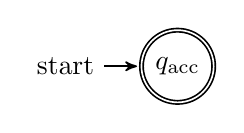
\begin{tikzpicture}[->,>=stealth',shorten >=1pt, auto, node distance=2cm, semithick]
  \tikzstyle{every state}=[text=black, fill=none]
  \node[initial,state,accepting] (q0)                    {$q_{\mathrm{acc}}$};
 ;
\end{tikzpicture}}
$, \varepsilon \rangle$}  
& \text{if } x = \langle M, w \rangle \text{ for a Turing machine $M$ and string $w$}\\
& \qquad \qquad \text{ and } w \in L(M) \\

\scalebox{.7}{$\langle$ \hspace{-.5cm} \raisebox{-.4cm}{
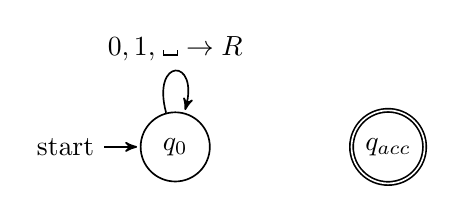
\begin{tikzpicture}[->,>=stealth',shorten >=1pt, auto, node distance=2cm, semithick]
  \tikzstyle{every state}=[text=black, fill=none]
  \node[initial,state] (q0)                    {$q_0$};
  \node[state,accepting] (qacc) [right of = q0, xshift = 20]{$q_{acc}$};
  \path (q0) edge  [loop above] node {$0, 1, \blank \to R$} (q0)
 ;
\end{tikzpicture}}
$\rangle$} 
& \text{otherwise}
\end{cases} 
\]


\item\gradeComplete $A_{\mathrm{TM}} \le_m EQ_{\mathrm{TM}} $ with 
\[
f(x) = \begin{cases}
 \scalebox{.7}{$\langle$ \hspace{-.5cm} \raisebox{-.4cm}{
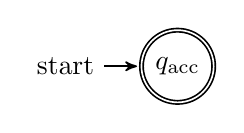
\begin{tikzpicture}[->,>=stealth',shorten >=1pt, auto, node distance=2cm, semithick]
  \tikzstyle{every state}=[text=black, fill=none]
  \node[initial,state,accepting] (q0)                    {$q_{\mathrm{acc}}$};
 ;
\end{tikzpicture}}
, $M_w \rangle$}  & \text{if } x = \langle M, w \rangle \text{ for a Turing machine $M$ and string $w$}\\\\
\scalebox{.7}{$\langle$ \hspace{-.5cm} \raisebox{-.4cm}{
    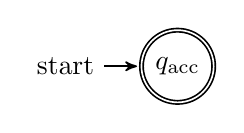
\begin{tikzpicture}[->,>=stealth',shorten >=1pt, auto, node distance=2cm, semithick]
      \tikzstyle{every state}=[text=black, fill=none]
      \node[initial,state,accepting] (q0)                    {$q_{\mathrm{acc}}$};
     ;
    \end{tikzpicture}}}
    , ~~~
    \scalebox{.7}{\hspace{-.5cm} \raisebox{-.4cm}{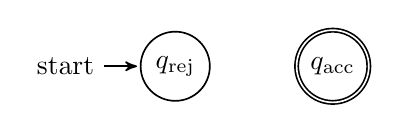
\begin{tikzpicture}[->,>=stealth',shorten >=1pt, auto, node distance=2cm, semithick]
        \tikzstyle{every state}=[text=black, fill=none]
        \node[initial,state] (qrej)                    {$q_{\mathrm{rej}}$};
        \node[state,accepting] (qacc) [right of=qrej]            {$q_{\mathrm{acc}}$};
       ;
      \end{tikzpicture}}$\rangle$ }  & \text{otherwise}.
\end{cases}
\]
Where for each Turing machine $M$, we  define 
\begin{align*}
    M_w = ``&\text{On input } y \\
    &1. \text{   Simulate $M$ on $w$.}\\
    &2. \text{   If it accepts, accept.}\\
    &3. \text{   If it rejects, reject."}
\end{align*}

\item\gradeCorrectFirst $HALT_{\mathrm{TM}} \le_m EQ_{\mathrm{TM}} $ with 
\[
f(x) = \begin{cases}
 \scalebox{.7}{$\langle$ \hspace{-.5cm} \raisebox{-.4cm}{
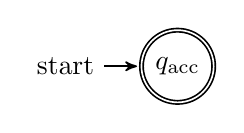
\begin{tikzpicture}[->,>=stealth',shorten >=1pt, auto, node distance=2cm, semithick]
  \tikzstyle{every state}=[text=black, fill=none]
  \node[initial,state,accepting] (q0)                    {$q_{\mathrm{acc}}$};
 ;
\end{tikzpicture}}
, $M_w \rangle$}  & \text{if } x = \langle M, w \rangle \text{ for a Turing machine $M$ and string $w$}\\\\
\scalebox{.7}{$\langle$ \hspace{-.5cm} \raisebox{-.4cm}{
    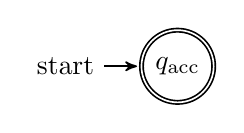
\begin{tikzpicture}[->,>=stealth',shorten >=1pt, auto, node distance=2cm, semithick]
      \tikzstyle{every state}=[text=black, fill=none]
      \node[initial,state,accepting] (q0)                    {$q_{\mathrm{acc}}$};
     ;
    \end{tikzpicture}}}
    , ~~~
    \scalebox{.7}{\hspace{-.5cm} \raisebox{-.4cm}{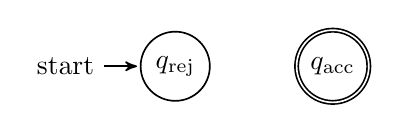
\begin{tikzpicture}[->,>=stealth',shorten >=1pt, auto, node distance=2cm, semithick]
        \tikzstyle{every state}=[text=black, fill=none]
        \node[initial,state] (qrej)                    {$q_{\mathrm{rej}}$};
        \node[state,accepting] (qacc) [right of=qrej]            {$q_{\mathrm{acc}}$};
       ;
      \end{tikzpicture}}$\rangle$ }  & \text{otherwise}.
\end{cases}
\]
Where for each Turing machine $M$, we  define 
\begin{align*}
    M_w = ``&\text{On input } y \\
    &1. \text{   If } y \text{ is not the empty string, reject.}\\
    &2. \text{   Else, simulate $M$ on $w$.}\\
    &3. \text{   If it accepts, accept.}\\
    &4. \text{   If it rejects, reject."}
\end{align*}

\item\gradeCorrect $\{w w \mid w \in \{0,1\}^* \} \leq \emptyset$ and
$f(x) = 1$ for each $x \in \{0,1\}^*$.

\item\gradeCorrect $\emptyset \le_m \{w w \mid w \in \{0,1\}^* \}$ and
$f(x) = 1$ for each $x \in \{0,1\}^*$.


\end{enumerate}

%%%%%%%%%%% PROBLEM 2 %%%%%%%%%%%
\item\textbf{Using mapping reductions} (14 points):
Consider the following computational problems we've discussed
\begin{align*}
A_{TM} &= \{ \langle M, w \rangle \mid M \text{ is a Turing machine, } w \text{ is a string and $M$ accepts $w$}\} \\
HALT_{TM} &= \{ \langle M, w \rangle \mid M \text{ is a Turing machine, } w \text{ is a string and $M$ halts on $w$}\} \\
E_{TM} &=  \{ \langle M \rangle \mid M \text{ is a Turing machine and } L(M) = \emptyset\} \\
EQ_{TM} &= \{ \langle M_1, M_2 \rangle \mid M_1, M_2 \text{ are both Turing machines and } L(M_1) = L(M_2) \}
\end{align*}
and the new computational problem
\[
    Two_{TM} = \{ \langle M \rangle \mid M \text{ is a Turing machine and $M$ accepts exactly one string} \}
\]

\begin{enumerate}
\item[(a)] \gradeCorrect Give an example of a string that is an element of $Two_{TM}$ and a string that is not an element of
$Two_{TM}$ and briefly justify your choices.
\item[(b)] \gradeComplete Prove that $Two_{TM}$ is not decidable by showing that $A_{TM} \leq_m Two_{TM}$.
\item[(c)] \gradeCorrect Give a different proof that $Two_{TM}$ is not decidable by showing that $HALT_{TM} \leq_m Two_{TM}$.
\item[(d)] \gradeComplete Is $Two_{TM}$ recognizable? Justify your answer.
\end{enumerate}

%%%%%%%%%%% PROBLEM 3 %%%%%%%%%%%
\item\textbf{Using mapping reductions} (14 points):
Consider the following computational problems we've discussed
\begin{align*}
A_{TM} &= \{ \langle M, w \rangle \mid M \text{ is a Turing machine, } w \text{ is a string and $M$ accepts $w$}\} \\
HALT_{TM} &= \{ \langle M, w \rangle \mid M \text{ is a Turing machine, } w \text{ is a string and $M$ halts on $w$}\} \\
E_{TM} &=  \{ \langle M \rangle \mid M \text{ is a Turing machine and } L(M) = \emptyset\} \\
EQ_{TM} &= \{ \langle M_1, M_2 \rangle \mid M_1, M_2 \text{ are both Turing machines and } L(M_1) = L(M_2) \}
\end{align*}
and the new computational problem
\begin{align*}
    Evens_{TM} &= \{ \langle M \rangle \mid M \text{ is a Turing machine 
    and any string that $M$ accepts must be even length}\\
    &\text{(but there may even length strings that $M$ doesn't accept)} \}
\end{align*}
\begin{enumerate}
\item[(a)] \gradeCorrect Give an example of a string that is an element of $Evens_{TM}$ and a string that is not an element of
$Evens_{TM}$ and briefly justify your choices.
\item[(b)] \gradeComplete Prove that $Evens_{TM}$ is not decidable by showing that $HALT_{TM} \leq_m Evens_{TM}$.
\item[(c)] \gradeCorrect Give a different proof that $Evens_{TM}$ is not decidable by showing that $A_{TM} \leq_m Evens_{TM}$.
\item[(d)] \gradeComplete Is $Evens_{TM}$ recognizable? Justify your answer.
\end{enumerate}


%%%%%%%%%%% PROBLEM 4 %%%%%%%%%%%
\item \textbf{Examples of languages} (7 points):

For each part of the question, use precise mathematical notation or English to define your examples
and then briefly justify why they work.

\begin{enumerate}
    \item\gradeCorrect Two undecidable languages $L_1$ and $L_2$ over the same alphabet
        whose intersection $L_1 \cup L_2$ is decidable, or write {\bf NONE}
        if there is no such example (and explain why).
    
    \item\gradeCorrect A regular language $L_3$ and an unrecognizable
        language $L_4$ over the same alphabet whose set-wise concatenation $L_3 \circ L_4$ is unrecognizable, 
        or write {\bf NONE} if there is no such example (and explain why).
    
    
    \item\gradeComplete A co-recognizable language $L_5$ that is NP-complete,
         or write {\bf NONE} if there is no such example (and explain why).
        Recall the definition: A language $L$ over an  alphabet $\Sigma$ is called {\bf co-recognizable} if its complement,  defined
        as $\Sigma^* \setminus L  = \{ x  \in  \Sigma^* \mid x \notin  L \}$, is Turing-recognizable.
        
\end{enumerate}
    

\end{enumerate}
\newpage
\titleformat{\subsubsection}[runin]
   {\normalfont\bfseries}{}{}{}
   
\title{ProjectCSE105F24: Project}
\date{Due December 11, 2024 at 11am}


\maketitle

\thispagestyle{fancy}


The CSE 105 project is designed for you to go deeper and 
extend your work on assignments 
and to see how some of the abstract notions we discuss can 
be implemented in concrete ways. 
The project is an individual assignment and has two tasks: 

Task 1: Illustrating the decidability of a computational problem, and

Task 2: Illustrating a mapping reduction

\subsubsection*{What resources can you use?} This project must be completed individually, 
without any help from other people, including the course staff (other than logistics support if 
you get stuck with screencast).
You can use any of this quarter's CSE 105 offering (notes, readings, class videos, homework feedback). 
Tools for drawing state diagrams (like Flap.js and JFLAP and the PrairieLearn automata library) can be used to help draw the diagrams 
in the project too.

These resources should be more than enough.
If you are struggling to get started and want to look elsewhere online, 
you must acknowledge this by listing and citing any resources you consult 
(even if you do not explicitly quote them), including any large-language model style resources (ChatGPT, Bard, Co-Pilot, etc.). 
Link directly to them and include the name of the author / video creator, 
any and all search strings or prompts you used, and the reason you consulted this reference. The work you submit for the project needs to be your own. Again, you shouldn't need to look anywhere 
other than this quarter's material and doing so may result in definitions that
conflict with our conventions in this class so think carefully before you go down this path.

If you get stuck on any part of the project, we encourage you to focus on communicating what you think 
the question might mean, including bringing an example from class or homework you think might be relevant, and 
include any submission any aspect where you're unsure. Clear communication about these
theoretical ideas and their applications is one of the main goals of the project.

{\bf Submitting the project} You will submit a PDF plus a video file for the first task and a PDF plus a video fiile for the 
second task. All file submissions will be in Gradescope.

\newpage
\subsubsection*{Your video:} You may produce screencasts 
with any software you choose. 
One option is to record yourself with Zoom; a tutorial on how to use 
Zoom to record a 
screencast (courtesy of Prof. Joe Politz)  is here: 

\url{https://drive.google.com/open?id=1KROMAQuTCk40zwrEFotlYSJJQdcG_GUU}.

The video that was produced from that recording session in Zoom is here:

\url{https://drive.google.com/open?id=1MxJN6CQcXqIbOekDYMxjh7mTt1TyRVMl}

Please send an email to the instructors 
(minnes@ucsd.edu) if you have 
concerns about  the video / screencast components of this project or 
cannot complete projects in this style for some reason.


\subsubsection*{Reference definitions for computational problems from Section 4.1:}
\begin{center}
   \begin{tabular}{|p{1in}cl|}
   \hline
   \multicolumn{3}{|l|}{{\bf  Acceptance problem} } \\
   & & \\
   \ldots for DFA & $A_{DFA}$ & $\{ \langle B,w \rangle \mid  \text{$B$ is a  DFA that accepts input 
   string $w$}\}$ \\
   \ldots for NFA & $A_{NFA}$ & $\{ \langle B,w \rangle \mid  \text{$B$ is a  NFA that accepts input 
   string $w$}\}$ \\
   \ldots for regular expressions & $A_{REX}$ & $\{ \langle R,w \rangle \mid  \text{$R$ is a  regular
   expression that generates input string $w$}\}$ \\
   \ldots for CFG & $A_{CFG}$ & $\{ \langle G,w \rangle \mid  \text{$G$ is a context-free grammar 
   that generates input string $w$}\}$ \\
   \ldots for PDA & $A_{PDA}$ & $\{ \langle B,w \rangle \mid  \text{$B$ is a PDA that accepts input string $w$}\}$ \\
   & & \\
   \hline
   \multicolumn{3}{|l|}{{\bf Language emptiness  testing} } \\
   & & \\
   \ldots for DFA & $E_{DFA}$ & $\{ \langle A \rangle \mid  \text{$A$ is a  DFA and  $L(A) = \emptyset$\}}$ \\
   \ldots for NFA & $E_{NFA}$ & $\{ \langle A\rangle \mid  \text{$A$ is a NFA and  $L(A) = \emptyset$\}}$ \\
   \ldots for regular expressions & $E_{REX}$ & $\{ \langle R \rangle \mid  \text{$R$ is a  regular
   expression and  $L(R) = \emptyset$\}}$ \\
   \ldots for CFG & $E_{CFG}$ & $\{ \langle G \rangle \mid  \text{$G$ is a context-free grammar 
   and  $L(G) = \emptyset$\}}$ \\
   \ldots for PDA & $E_{PDA}$ & $\{ \langle A \rangle \mid  \text{$A$ is a PDA and  $L(A) = \emptyset$\}}$ \\
   & & \\
   \hline
   \multicolumn{3}{|l|}{{\bf Language equality testing} } \\
   & & \\
   \ldots for DFA & $EQ_{DFA}$ & $\{ \langle A, B \rangle \mid  \text{$A$ and $B$ are DFAs and  $L(A) =L(B)$\}}$\\
   \ldots for NFA & $EQ_{NFA}$ & $\{ \langle A, B \rangle \mid  \text{$A$ and $B$ are NFAs and  $L(A) =L(B)$\}}$\\
   \ldots for regular expressions & $EQ_{REX}$ & $\{ \langle R, R' \rangle \mid  \text{$R$ and $R'$ are regular
   expressions and  $L(R) =L(R')$\}}$\\
   \ldots for CFG & $EQ_{CFG}$ & $\{ \langle G, G' \rangle \mid  \text{$G$ and $G'$ are CFGs and  $L(G) =L(G')$\}}$ \\
   \ldots for PDA & $EQ_{PDA}$ & $\{ \langle A, B \rangle \mid  \text{$A$ and $B$ are PDAs and  $L(A) =L(B)$\}}$ \\
   \hline
   \end{tabular}
   \end{center}


\newpage
\subsubsection*{Task 1: Illustrating the decidability of a computational problem}

Many computational problems are decidable, sometimes using beautiful algorithms.
In this part of the project, you'll choose a 
{\bf decidable} computational problem, and demonstrate the proof that it is 
decidable by building a program in a programming language of your choice (aka a high-level description of a Turing machine) that decides it. 
You will then demonstrate  how your construction works for some test examples.

Specifically:

\vspace{-10pt}

\begin{enumerate}
\item Choose a decidable computational problem from Section 4.1. 
{\it Note:
if you'd like to consider a different computational problem instead, please check with Prof. Minnes first. You must do so no later than the start of Week 9.}
\item Write a program in Java, Python, JavaScript, C++ , or another programming language of your choosing that decides this computational problem.  The function input must be a {\bf string} and part of your work in this program 
is to design string representations for arbitrary instances of the model of 
computation the computational problem you picked is about (e.g. DFA, NFA, regular expressions, CFG, or NFA). The function output must be a {\bf boolean} 
true (if the string is in the set representing the computational problem) or 
false (if the string is not in the set representing the computational problem).
\begin{itemize}
   \item You may use our class notes and the textbook for ideas on the algorithm that your program will implement.
   \item If you would like, you may use aids such as co-pilot or ChatGPT to help you write this program. 
   However, you should test the code that is produced and be able to explain what it is doing. Your code needs to be well-organized and well-documented.
   As a header in your code file, include a comment block describing any resources that were used to 
   help generate your code, including any and all prompts used in interactions 
   with LLM coding tools.
\end{itemize}

\item To demonstrate your program, select one string that is in the 
set representing the computational problem, and one string that is not in the 
set representing the computational problem, explain why these strings are valid
examples, and demonstrate running your program on each to get the appropriate 
output.
\end{enumerate}

Presenting your reasoning and demonstrating it via screenshare are important 
skills that also  show us a lot of your learning. Getting practice with this 
style of presentation is a good thing  for you to learn in general and a rich 
way for us to assess your skills. 
To demonstrate your work, you will create a 3-5 minute screencast video 
explaining your code design and demonstrating its functionality.

\newpage
{\bf Checklist for submission} For this task, you will submit a PDF plus a video file.

\vspace{-10pt}

\begin{itemize}
   \item[(PDF)] Writeup includes a clear specification of computational problem being decided.
   \item[(PDF)] Documentation for program deciding this computational problem: 
   include a description of how input strings are parsed to represent
   instances of the computational problem.
   \item[(PDF)] Clear specification of two example strings, explaining which is in the set (and why) and which is not in the set (and why not).
   \item[(PDF)] Project submission includes a printout of code for program implementing algorithm to decide the computational problem, as well as screen shots demonstrating running your program on your 
   example strings.
   \item[(PDF)] Project writeup is typed or clearly hand drawn with precise language and notation for all terms.
   \item[(Video)] Start with your face and your student ID visible for a few seconds at the beginning, and introduce yourself audibly while on screen. You don't have to be on camera for the  rest of the video, though it's fine if you are. We are looking for a brief confirmation that  it's you creating the video and doing the work you submitted.
\item[(Video)] Present the computational problem you will be working with, and 
example strings that you will be using, including explanations of why you chose this problem and these strings (and why one of the strings is in the set 
and why the other is not).
\item[(Video)] Show on the screen and explain the code for your program, including the software design choices you made
(e.g. which data structures are you using, etc.) and any resources you used. The video 
should clearly describe which programming language was chosen 
for the implementation and gives the reasons why.
\item[(Video)] Demonstrate running your code on each of your example inputs. The video should include screencasts of 
running the code live.
Explain why the output of your program is what you would expect, by connecting the output of the the definition of the computational problem and your chosen parsing of input strings.
\item[(Video)] Logistics: video needs to load correctly, be between 3 and 5 minutes, 
show your face and ID, and you introduce yourself 
audibly while on screen.
\end{itemize}

{\bf Note}: Clarity and brevity are both important aspects of your video.  In previous years, we've seen 
students speed up their videos to get below the 5 minute upper bound. This is ok so long as it doesn't 
compromise clarity. If the graders need to slow your video down to understand
it, it may not earn full credit.


\newpage
\subsubsection*{Task 2: Illustrating a mapping reduction}

We can use mapping reductions to prove that interesting computational 
problems are undecidable, building on 
the undecidability of other computational problems.
In this part of the project, you'll choose a specific {\bf mapping reduction}
and implement a computable function that witnesses it
using a  programming language of your choice (aka a high-level description of a Turing machine that computes it).
You will then demonstrate  how your construction works for some test examples.

Specifically:

\vspace{-10pt}

\begin{enumerate}
\item Choose a mapping reduction we discussed in class or in the homework
or in review quizzes or in the textbook where both sets being compared are 
undecidable. {\it Note:
if you'd like to consider a  mapping reduction we have not discussed instead, 
please check with Prof. Minnes first. 
You must do so no later than the start of Week 9.}
\item Write a program in Java, Python, JavaScript, C++ , or another programming language of your choosing that implements a computable function witnessing this mapping reduction.  The function input must be a {\bf string}  and the function 
output must be a {\bf string}. Part of your work in this program 
is to design string representations for arbitrary instances of the model of 
computation the computational problems being compared in the mapping reduction.
Your function will need to be able to process *any* string as input.
\begin{itemize}
   \item You may use our class notes and the textbook for ideas on the algorithm that your program will implement.
   \item If you would like, you may use aids such as co-pilot or ChatGPT to help you write this program. 
   However, you should test the code that is produced and be able to explain what it is doing. Your code needs to be well-organized and well-documented.
   As a header in your code file, include a comment block describing any resources that were used to 
   help generate your code, including any and all prompts used in interactions 
   with LLM coding tools.
\end{itemize}

\item To demonstrate your program, you will need to run it for an example positive and negative instance. That is to say, if you are implementing 
a computable function witnessing $X \leq_m Y$, you will select one string that is in $X$ and one string that is not in $X$, and you will 
 demonstrate running your program on each of these strings and explain why 
 the output of the function is good.
\end{enumerate}

Presenting your reasoning and demonstrating it via screenshare are important 
skills that also  show us a lot of your learning. Getting practice with this 
style of presentation is a good thing  for you to learn in general and a rich 
way for us to assess your skills. 
To demonstrate your work, you will create a 3-5 minute screencast video 
explaining your code design and demonstrating its functionality.

\newpage
{\bf Checklist for submission} For this task, you will submit a PDF plus a video file.

\vspace{-10pt}

\begin{itemize}
   \item[(PDF)] Writeup includes a clear specification of mapping reduction being witnessed, and both sets in the reduction are undecidable.
   \item[(PDF)] Documentation for program computing the function witnessing this mapping reduction:
   include a description of how input strings are parsed and how output strings correspond to input strings.
   \item[(PDF)] Clear specification of two example strings, explaining which is is a positive instance (and why) and which is a negative instance (and why not).
   \item[(PDF)] Project submission includes a printout of code for program computing the function witnessing the mapping reduction, as well as screen shots demonstrating running your program on your 
   example strings.
   \item[(PDF)] Project writeup is typed or clearly hand drawn with precise language and notation for all terms.
   \item[(Video)] Start with your face and your student ID visible for a few seconds at the beginning, and introduce yourself audibly while on screen. You don't have to be on camera for the  rest of the video, though it's fine if you are. We are looking for a brief confirmation that  it's you creating the video and doing the work you submitted.
\item[(Video)] Present the mapping reduction you will be working with, and 
example strings that you will be using, including explanations of why you chose this reduction and these strings (and why one of the strings is a positive instance and the other is a negative instance).
\item[(Video)] Show on the screen and explain the code for your program, including the software design choices you made
(e.g. which data structures are you using, etc.) and any resources you used. The video 
should clearly describe which programming language was chosen 
for the implementation and gives the reasons why.
\item[(Video)] Demonstrate running your code on each of your example inputs. The video should include screencasts of 
running the code live.
Explain why the output of your program is what you would expect, by connecting the output of the 
program to the definition of the mapping reduction and your chosen parsing of input strings.
\item[(Video)] Logistics: video needs to load correctly, be between 3 and 5 minutes, 
show your face and ID, and you introduce yourself 
audibly while on screen.
\end{itemize}

{\bf Note}: Clarity and brevity are both important aspects of your video.  In previous years, we've seen 
students speed up their videos to get below the 5 minute upper bound. This is ok so long as it doesn't 
compromise clarity. If the graders need to slow your video down to understand
it, it may not earn full credit.



\newpage

\end{document}